\documentclass{article}[18pt]
\ProvidesPackage{format}
%Page setup
\usepackage[utf8]{inputenc}
\usepackage[margin=0.7in]{geometry}
\usepackage{parselines} 
\usepackage[english]{babel}
\usepackage{fancyhdr}
\usepackage{titlesec}
\hyphenpenalty=10000

\pagestyle{fancy}
\fancyhf{}
\rhead{Sam Robbins}
\rfoot{Page \thepage}

%Characters
\usepackage{amsmath}
\usepackage{amssymb}
\usepackage{gensymb}
\newcommand{\R}{\mathbb{R}}

%Diagrams
\usepackage{pgfplots}
\usepackage{graphicx}
\usepackage{tabularx}
\usepackage{relsize}
\pgfplotsset{width=10cm,compat=1.9}
\usepackage{float}

%Length Setting
\titlespacing\section{0pt}{14pt plus 4pt minus 2pt}{0pt plus 2pt minus 2pt}
\newlength\tindent
\setlength{\tindent}{\parindent}
\setlength{\parindent}{0pt}
\renewcommand{\indent}{\hspace*{\tindent}}

%Programming Font
\usepackage{courier}
\usepackage{listings}
\usepackage{pxfonts}

%Lists
\usepackage{enumerate}
\usepackage{enumitem}

% Networks Macro
\usepackage{tikz}


% Commands for files converted using pandoc
\providecommand{\tightlist}{%
	\setlength{\itemsep}{0pt}\setlength{\parskip}{0pt}}
\usepackage{hyperref}

% Get nice commands for floor and ceil
\usepackage{mathtools}
\DeclarePairedDelimiter{\ceil}{\lceil}{\rceil}
\DeclarePairedDelimiter{\floor}{\lfloor}{\rfloor}

% Allow itemize to go up to 20 levels deep (just change the number if you need more you madman)
\usepackage{enumitem}
\setlistdepth{20}
\renewlist{itemize}{itemize}{20}

% initially, use dots for all levels
\setlist[itemize]{label=$\cdot$}

% customize the first 3 levels
\setlist[itemize,1]{label=\textbullet}
\setlist[itemize,2]{label=--}
\setlist[itemize,3]{label=*}

% Definition and Important Stuff
% Important stuff
\usepackage[framemethod=TikZ]{mdframed}

\newcounter{theo}[section]\setcounter{theo}{0}
\renewcommand{\thetheo}{\arabic{section}.\arabic{theo}}
\newenvironment{important}[1][]{%
	\refstepcounter{theo}%
	\ifstrempty{#1}%
	{\mdfsetup{%
			frametitle={%
				\tikz[baseline=(current bounding box.east),outer sep=0pt]
				\node[anchor=east,rectangle,fill=red!50]
				{\strut Important};}}
	}%
	{\mdfsetup{%
			frametitle={%
				\tikz[baseline=(current bounding box.east),outer sep=0pt]
				\node[anchor=east,rectangle,fill=red!50]
				{\strut Important:~#1};}}%
	}%
	\mdfsetup{innertopmargin=10pt,linecolor=red!50,%
		linewidth=2pt,topline=true,%
		frametitleaboveskip=\dimexpr-\ht\strutbox\relax
	}
	\begin{mdframed}[]\relax%
		\centering
		}{\end{mdframed}}



\newcounter{lem}[section]\setcounter{lem}{0}
\renewcommand{\thelem}{\arabic{section}.\arabic{lem}}
\newenvironment{defin}[1][]{%
	\refstepcounter{lem}%
	\ifstrempty{#1}%
	{\mdfsetup{%
			frametitle={%
				\tikz[baseline=(current bounding box.east),outer sep=0pt]
				\node[anchor=east,rectangle,fill=blue!20]
				{\strut Definition};}}
	}%
	{\mdfsetup{%
			frametitle={%
				\tikz[baseline=(current bounding box.east),outer sep=0pt]
				\node[anchor=east,rectangle,fill=blue!20]
				{\strut Definition:~#1};}}%
	}%
	\mdfsetup{innertopmargin=10pt,linecolor=blue!20,%
		linewidth=2pt,topline=true,%
		frametitleaboveskip=\dimexpr-\ht\strutbox\relax
	}
	\begin{mdframed}[]\relax%
		\centering
		}{\end{mdframed}}
\lhead{CSys}


\begin{document}
\begin{center}
\underline{\huge Addressing Modes}
\end{center}
\section{CPU Fetch Execute Cycle}
\begin{enumerate}
	\item CPU sends the address in the program counter (PC) to the Memory Address Register (MAR)
	\item Increment the PC
	\item Get the instruction identified by the MAR into the Memory Data Register (MDR)
	\item Move the instruction from the MDR to the instruction register
	\item Move the instruction from the IR to the control unit for \textbf{decoding}
	\begin{itemize}
		\item Send the operation to the ALU
		\item Put the address if data to be operated upon in a register
	\end{itemize}
	\item Send the address if data to be operated upon in a register
	\item Read the data from memory into the MDR
	\item Move the data from the MDR to an accumulator into the ALU
	\item Do the operation and store the result in an accumulator in the ALU	
	
\end{enumerate}
\section{Addressing}
Sometimes we would like to:
\begin{itemize}
	\item Address a large amount of memory with only a few bits
	\item Use indexes to loop or examine a table or array
	\item Relocate data or programs in the memory
	\item Operate on the registers rather than actual memory
\end{itemize}
This can be achieved using alternative addressing modes\\
\\
Sometimes we don't know where exactly we want to index to, but instead know the relative position to where you currently are.
\subsection{Alternatives to direct addressing}
\begin{itemize}
	\item \textbf{Direct addressing} - the address read in the instruction is the address of the actual data
	\item \textbf{Immediate addressing} - the address read in the instruction \textbf{is the data} to be used. Suitable for constants, e.g. add 1
	\item \textbf{Indirect addressing} - the address read in the instruction is the address of a memory location containing the address of the actual data
	\item \textbf{Register indirect addressing} - the address read in the instruction is the address of a register containing the address of the actual data
	\item \textbf{Indexed addressing} - the address read in the instruction should have an index value (contained in some register) added to obtain the address of the data
\end{itemize}
\section{Adding a column}
\subsection{Direct}
\begin{itemize}
	\item The instruction in a specific address is changed during the program
	\item This is called \textbf{impure code} - pure code does not change when it is run
	\item It can cause difficulties:
	\begin{itemize}
		\item If the index is not reset, next time the program will run differently
		\item If the program is interrupted the address will not be reset
		\item The program cannot be run from ROM
	\end{itemize}
\end{itemize}
\subsection{Indirect}
Loop over a table, and increment a value each time

\subsection{Indexed}
\begin{center}
	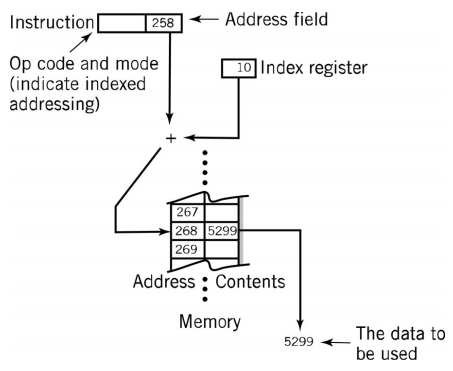
\includegraphics[scale=0.7]{indexed}
\end{center}
\begin{center}
	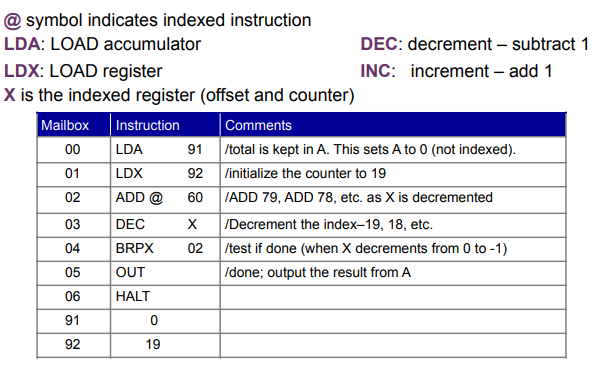
\includegraphics[scale=0.7]{indexed1}
\end{center}
Note the index is decremented each time
\section{Addressing mode}
We used * and @ to indicate addressing mode\\
In a real CPU, the \textbf{instruction itself} will need to contain the addressing mode
\section{Alternative to absolute addressing}
\textbf{Absolute} - The address read is the one the minion should go to (except for indexed addressing)\\
\textbf{Relative addressing} - The address read is an offset to the current instruction address
\begin{center}
	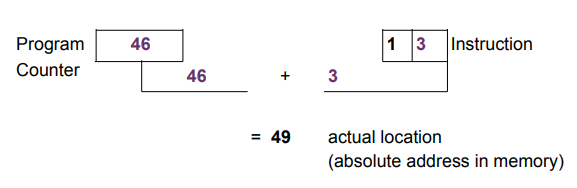
\includegraphics[scale=0.7]{alternative}
\end{center}
\textbf{Base offset addressing} - the address read is offset by the current value in a special 'base' register
\begin{center}
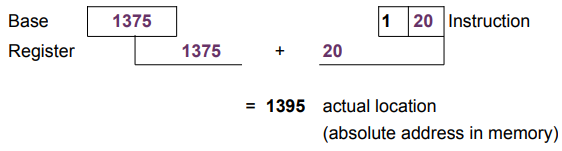
\includegraphics[width=0.7\linewidth]{alternative1}
\end{center}
\textbf{IBM zSystem Load instruction:}
\begin{center}
	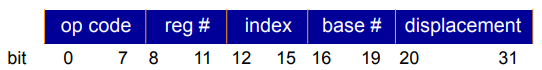
\includegraphics[scale=0.7]{alternative2}
\end{center}
\begin{center}
	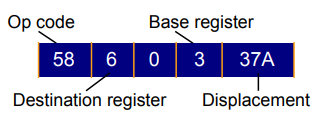
\includegraphics[scale=0.7]{alternative3}
\end{center}
\section{Instructions}
\subsection{Data movement}
Movement of data between:
\begin{itemize}
	\item Registers
	\item Registers and memory
	\item Memory locations (infrequently)
\end{itemize}
The most heavily used part of an instruction set and therefore it must be the most flexible, using different sizes of data\\
\subsection{Arithmetic Instructions:}
Most modern CPU's instruction set includes:
\begin{itemize}
	\item Integer addition and subtraction
	\item Integer multiplication and division
	\item Floating point instructions
\end{itemize}
\subsection{Program control:}
\begin{itemize}
	\item JUMPS
	\item BRANCHES (Conditional or Unconditional)
	\item CALL
	\item RETURN
\end{itemize}
\subsection{Boolean logic instructions:}
\begin{itemize}
	\item \textbf{Bit manipulation}
	\begin{itemize}
		\item Allows programmers to control program flow by providing the mechanism for them to design their own 'flags'
		\item Instructions include set and test
	\end{itemize}
	\item \textbf{Shift and Rotate Instructions}
	\begin{itemize}
		\item Shift: Move data bits left or right one or more bits at a time. Bits shifted out of the end may trigger a flag or drop off the end. Fill in with 0s
		\item Rotate: move data bits left or right one of more bits at a time. Bits shifted to the end are rotated back to the beginning. Loop round
	\end{itemize}
\end{itemize}
\subsection{Single operand manipulation}
\begin{itemize}
	\item Negating a value
	\item Incrementing a value
	\item Decrementing a value
	\item Setting a register to zero
\end{itemize}
\subsection{Multiple data instructions}
\subsection{Stack instructions}
\begin{itemize}
	\item POP
	\item PUSH
\end{itemize}
\end{document}